\section{Problem Overview}
\label{sec:overview}

The scope of the problem can be thought of as follows: we aim to integrate data analytics within
a document in a manner that maximizes the ability of the reader to understand the core information
being presented. Existing solutions such as notebooks and literate programming are limited by their
labour-intensive nature, and the lack of interactivity between data visualizations and accompanying text.

This large scale problem is a difficult one, there are many sub-problems that do not have immediate answers.
Two of the main issues are scale and abstraction: modern data analysts employ complex models and large datasets.
Bridging the gap between -- for example -- the results of a regression analysis and the natural language description
of the results is difficult, due to the presence of steps like feature-selection. Furthermore with modern approaches
such as neural networks, the analytical methods themselves can become black-boxes.

Automating this process would require a system that can generate code which correctly performs the data analysis,
which is a task well beyond the scope of current research in AI. We shall instead restrict our attention to a smaller
problem, namely how do we link text and visualizations based on the results of a data analysis that has already been
performed. The larger problem should be considered a long-term goal for such a research program.

\subsection{Linking Text To Visual and Data Objects}
We shall make the assumption that the author of an article has already written the code which performs
their data analysis, and the code which turns the results into useful visualisations. Restricting the scope to the problem of
automatically generating code which references the pre-computed visual and data objects.
Indeed, without having solved this more restricted problem it is difficult to see how one would approach
the more general problem of embedding data analytics directly into text.

\subsection{The Linguistic Sorts of Linked Text}
We begin by breaking down the sorts of linked text that the developer may
be interested in generating. 

\begin{figure}
   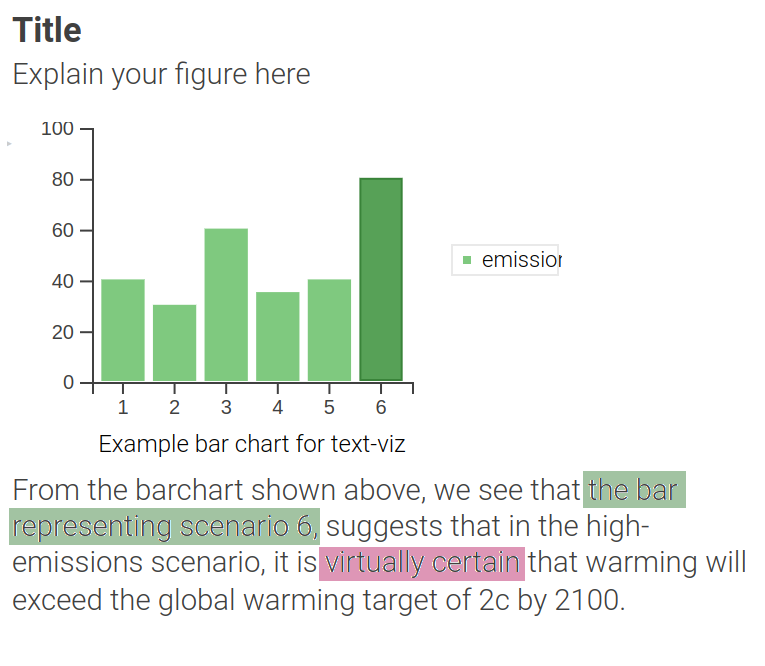
\includegraphics[width=0.7\textwidth]{fig/text-viz-types.png}
   \caption{Two sorts of linked text}
   \label{fig:linked-text-types}
\end{figure}

\subsubsection{Graded Adjectives}
A graded adjective is an adjective that can be modified to make its form stronger or weaker.
As an example, consider mapping ranges of probabilities onto natural language. If the probability
of an event occurring is $1$, we can say it is \emph{certain} to occur. If instead it is $0.99$
or some other value arbitrarily close to $1$, we will \emph{grade} the adjective to weaken it:
it is \emph{virtually certain} to occur. In \figref{linked-text-types}, this corresponds to the text
highlighted in pink.

\subsubsection{Indexing Visual Elements: Mereology}
Often, visualisations are paired with descriptions of the information the visualisation is attempting to
convey. Even when such text appears to make direct reference to a visual element, it can be unclear what 
it should specifically be linked against. For example, in \figref{linked-text-types}, the text highlighted
in green is referring to one of the bars in the chart, but it is not clear how this should be presented.
In the example, this information is communicated by highlighting the bar itself, but in a sense the text is
instead referencing the index of the bar rather than the bars contents. It could therefore be argued that the
the text should be linked against the index variable underneath the bar, rather than the bar itself.
Our system needs to be able to walk arbitrarily deep into nested structures when performing the linking.

This is an example of the more general linguistic problem of mereology: analysing relationships between the
whole and the parts from which it is composed. In the case of the chart, one can reference: the chart as a whole,
the bars as a whole, individual bars, the fields of the records underlying each of the bars, and so on.
We will need our system to be able to generate linked text that can make these arbitrary walks into the nested
data structures we provide.


\begin{figure}
   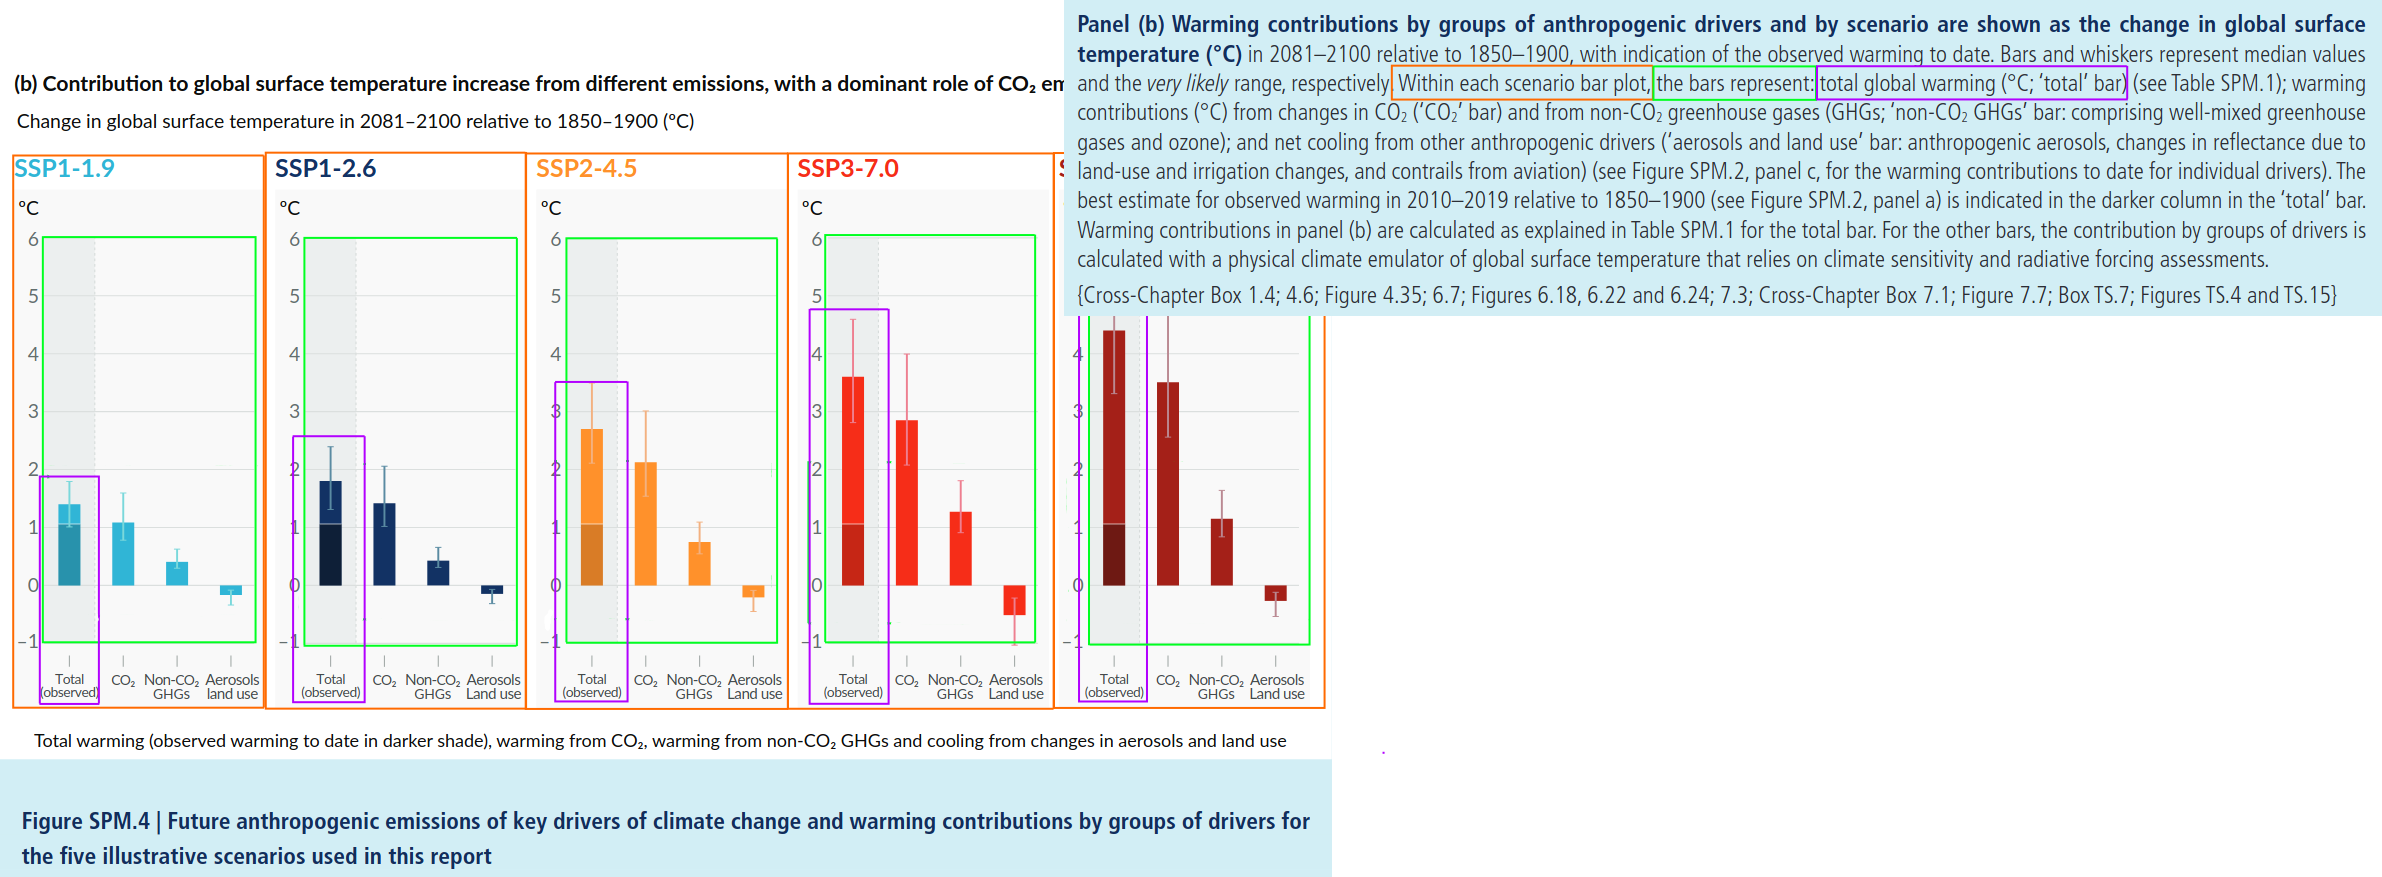
\includegraphics[width=0.7\textwidth]{fig/ipcc-visual-elements.png}
   \caption{Examples of scope in linked text}
   \label{fig:visual-element-scope}
\end{figure}

\subsubsection{Iterators and Scope}
The next linguistic form that our system must be able to work with is that of iteration and scope. 
In \figref{visual-element-scope}, the text highlighted with the first red box creates a scope for
the references that follow. The text which follows it refers to bars within an individual chart,
with the understanding that the references to these components are distributed across each chart
within the scope. In effect, the text can be thought of as mapping links over every chart in scope.

\subsubsection{Quantitative Expressions}
On its surface, directly embedding a quantitative expression into the text seems to be the simplest
of the linguistic categories we have identified thus far, but this may not be the case. Embedding
a percentage may be simple: requiring the user to only provide a numerical value, and scaling it
to be in the range of $0$-$100$, but more complicated expressions, such as a description of a calculation
may be more difficult to synthesize. 

\subsection{Applications of Self-Certifying Text}
Here we shall present some examples of the type of policy that we might want to synthesize.

\paragraph{Calibrated Terminology:} in scientific reporting, probabilities are often not directly given, but instead
mapped to calibrated terminology. We have already mentioned the term ``virtually certain'' from the IPCC report, but in the beginning
of that document, they make sure to explain the meaning of terms like ``likely'' and ``very likely'' as well. This
sort of simple conversion is an example of the simplest form of policy that one might want to synthesize.

\subsection{Challenges}
Applying language models to the task of code generation is not new, however the aim of generating code that
itself produces natural language appears to be a novel one. We currently anticipate the following challenges,
and will add more as the work progresses.

\paragraph{Small number of examples:} as a language, Fluid is incredibly niche, and so we have a very small corpus
of programs on which to train a language model. Further, we currently only have 2 example programs that actually make
use of the \kw{LinkedText} construct which we intend to use. The problem then is how to best make use of the capabalities
of current language models in this context. For example, should we perform some sort of few-shot learning or prompt-engineering
technique on a large pre-trained model, should we augment our corpus of training examples manually or both? If we take a meta-learning
perspective (\todo{CITE}), we may run into problems of the model preferring syntax and function names from the languages we use to
train the model.

\paragraph{Counter-intuitive dependency relation:} at the moment, dependencies that are computed by Fluid can be counter-intuitive.
Until we revamp the underlying dependency model, we will need to generate code that follows the pattern of ``consuming'' input
data in order to produce the output text. This may be a problem for things like generating direct references to visual elements.

\paragraph{Potentially complex code:} for many purposes, we want to store the data objects being referred to in variables. This 
could mean complicated code, and cluttering a source file. We will potentially need to find a general pattern for this sort of thing,
so that an authors document doesn't get filled with extraneous variable declarations. 